\documentclass[a4paper,11pt]{article}

\usepackage{mathtools}
\usepackage{lipsum}
\usepackage{fullpage}
\usepackage{tabu}
\usepackage{wrapfig}
\usepackage{array,ragged2e,pst-node,pst-dbicons}
\usepackage{graphicx}

\title{Computer System II Networks Assignment}
\date{\today}
\author{James King}

\begin{document}
\maketitle

\begin{abstract}
\emph{The Travelling Salesman Problem is an example of the NP-Complete class of
problems; attempting to find the optimal solution by trying every possibility
would require an obscene amount of time for all but the smallest of input
sizes. This report describes two methods for finding decent solutions in a 
reasonable amount of time. The first is a type of stochastic gradient descent,
and the second is a nature inspired algorithm that models a simple ant colony.
A piece of analysis software was also produced to try and display each given
input in a form that is understandable to humans.}
\end{abstract}

\section{General Data Structures}
Each city graph, after being loaded from an input file, is stored in a 2D
integer array in such a way that the value in column $i$ and row $j$ is the
distance between city $i$ and city $j$. Representing the graph in this form
meant that checking the distance between two cities is a simple and fast
operation, and I hoped this would lead to my search algorithms being more time
efficient.

Routes are represented as fixed length one dimensional integer arrays, with
each value in the array being the index of the associated city. Each route also
has two numbers stored inside it that record the number of cities in the route
and the total cost of the route (the sum of the distances between each city in
the route). The value for the route cost is initially set to $-1$, and when it
is requested and its value is $-1$ it recalculates this cost. Additionally, any
operations that could change the length of the route set this value back to
$-1$, signalling that the value needs to be recalculated when next requested.

When an empty route is first created, the values in its city array are the
indexes of each city in ascending order. When the $i$th city is added to the
route, the relevant index is swapped with the value that was at the $i$th
position. This means that for a route of length $j$, all values in the array
from $j+1$ onwards are the indexes of cities that are not currently in the tour
and therefore can be selected to be added to the tour. I have also provided the
facility of selecting the $k$th best city from this subset, using the end of
the array as a buffer which is partially ordered until the city that is $k$th
best using a given comparison criteria is found.

\section{Algorithms}
\subsection{Algorithm A}
Initially I wanted to create a simple deterministic improvement search
algorithm to use as a benchmark when testing the capabilities of more complex
algorithms. Not wanting to simply copy a method I found from the internet, I
attempted to find my own solution without researching existing ones.

Each improvement search algorithm must have at least one mutation method which
can be applied to a route. It should be possible, though multiple applications
of this mutation method, to mutate any valid route into any other valid route.
A gradient descent algorithm is a variant of the improvement search which will
only perform mutations that immediately improve the current route, and this is
the class of algorithm I intended to design.

My first task was to decide on a mutation method. The method would need to be
quite simple in order to test many different mutations in a small amount of
time to find which ones improve the tour. I opted for a mutator which selects
two cities in the tour and reverses the ordering of all cities between them.
This method satisfies the condition of being able to traverse the search space
between any two tours, given that swapping pairs of cities in the tour allows
for any permutation of tour to be explored. A swap can be performed through two
reversals, the first to swap the pair of cities you wish to exchange, and the
second to reverse the cities between then into their initial order. With this
reversal mutation method, it is also computationally simple to find how the
length of the tour will be affected. Because the connections between each pair
of cities inside the group being reversed will have the same cost (assuming the
graph is symmetric), only the two connections between the set of cities being
reversed and the rest of the tour will change in a way that could alter the
tour length. The amount by which a reversal between two cities $T_i$ and $T_j$
will affect the tour length is therefore:

$$(|\overrightarrow{{T_{i-1}}{T_i}}|
+ |\overrightarrow{{T_j}{T_{j+1}}}|)
- (|\overrightarrow{{T_{i-1}}{T_j}}|
+ |\overrightarrow{{T_i}{T_{j+1}}}|)$$

\noindent
Here $T_i$ is the $i$th city in tour $T$, and $|\overrightarrow{{T_i}{T_j}}|$
is the distance between city $T_i$ and $T_j$ as described by the city graph
given as input.

\begin{figure}
\begin{center}
\begin{tabular}{c}
\Large
\Circlenode[radius=4mm,linestyle=dashed]{f1start}{~}
\hskip 5mm
\Circlenode[radius=4mm]{f1A}{A} \ncline[linestyle=dashed]{f1start}{f1A}
\hskip 5mm
\Circlenode[radius=4mm]{f1B}{B} \ncline{f1A}{f1B}
\hskip 5mm
\Circlenode[radius=4mm]{f1C}{C} \ncline{f1B}{f1C}
\hskip 5mm
\Circlenode[radius=4mm]{f1D}{D} \ncline{f1C}{f1D}
\hskip 5mm
\Circlenode[radius=4mm]{f1E}{E} \ncline{f1D}{f1E}
\hskip 5mm
\Circlenode[radius=4mm]{f1F}{F} \ncline{f1E}{f1F}
\hskip 5mm
\Circlenode[radius=4mm]{f1G}{G} \ncline{f1F}{f1G}
\hskip 5mm
\Circlenode[radius=4mm,linestyle=dashed]{f1end}{~}
\ncline[linestyle=dashed]{f1G}{f1end}
\ncarc[arcangle=30,linestyle=dashed]{->}{f1B}{f1F}
\ncarc[arcangle=30,linestyle=dashed]{<-}{f1E}{f1A}
\\[1cm]
\Large
\Circlenode[radius=4mm,linestyle=dashed]{f2start}{~}
\hskip 5mm
\Circlenode[radius=4mm]{f2A}{A} \ncline[linestyle=dashed]{f2start}{f2A}
\hskip 5mm
\Circlenode[radius=4mm]{f2E}{E} \ncline{f2A}{f2E}
\hskip 5mm
\Circlenode[radius=4mm]{f2D}{D} \ncline{f2E}{f2D}
\hskip 5mm
\Circlenode[radius=4mm]{f2C}{C} \ncline{f2D}{f2C}
\hskip 5mm
\Circlenode[radius=4mm]{f2B}{B} \ncline{f2C}{f2B}
\hskip 5mm
\Circlenode[radius=4mm]{f2F}{F} \ncline{f2B}{f2F}
\hskip 5mm
\Circlenode[radius=4mm]{f2G}{G} \ncline{f2F}{f2G}
\hskip 5mm
\Circlenode[radius=4mm,linestyle=dashed]{f2end}{~}
\ncline[linestyle=dashed]{f2G}{f2end}
\end{tabular}
\end{center}
\caption{Segment of a tour before and after a reversal is applied between
	\emph{B} and \emph{E}, with the two new connections to be added represented
	by dashed arcs. The only connections that differ in cost to the original
	tour are the new connections from \emph{A} to \emph{E} and \emph{B} to
	\emph{F}.}
\end{figure}

I implemented the search as a greedy gradient descent, where for each iteration
the algorithm looks through all possible pairs of cities and chooses to reverse
between the ones that would lead to the biggest drop in tour size. This on its
own produced some decent results, and was extremely fast. I experimented by
combining it with a Best First Search, where for every new city added to the
tour by the BFS the reversing improvement algorithm would be executed. This
naturally produced smaller tours than either of the two algorithms on their
own, and due to its speed and the quality of the results I decided to take the
method further and see how I could improve it.

I noticed through experimentation that for some city graphs my combined 
algorithm actually produced a better result if the BFS was replaced by a 
\emph{Worst} First Search. This made me think that maybe it would be possible
for the algorithm to give even better results when using a stochastic
constructive search in the place of a Best or Worst First Search. Because the
reversal process was pretty fast, and constructing a tour by selecting random
cities would naturally be faster than checking each one to see if it was the
best or worst, I reasoned that I could test thousands of tours generated this
way in a short amount of time. This new method produced some new records for
a few of the city graphs the first time it was tested, and the more time it was
left running for the higher the probability of a new record. Adding the ability
for the method to utilize multiple threads meant that it would produce more
records in the same amount of time as before, and after a couple of weeks of
running it for a few minutes a day it seemed to reach a minimum for each city
graph that it was unlikely to improve on.

\subsection{Algorithm B}

Before I started work on my second method I wanted to have a go at visualising
the graphs in a way that attempts to portray the distances between each node,
thinking that with some extra insight into how the graphs were laid out I would
be able to think of better methods of solving the problem. I wrote a simple
program that essentially simulates springs between each city with strengths
related to the distance between each city pair, and allow the cities to move
until they are at an equilibrium. This method would work best for graphs where
each cost to travel between two cities was based on the euclidean distance
between two points that represent those cities.

\begin{wrapfigure}{r}{0.5\textwidth}
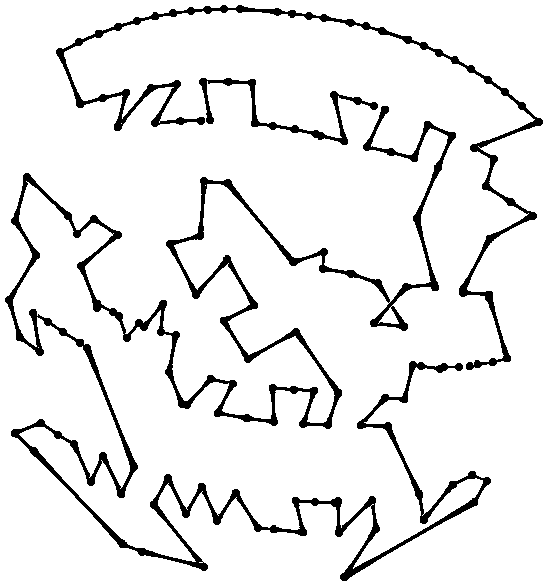
\includegraphics[width=0.48\textwidth]{175vis}
\caption{Visualisation of the 175 city graph with the current shortest route.}
\end{wrapfigure}

This worked much more successfully than I expected. I was anticipating all the
graphs having distances that were entirely random, and therefore not euclidean.
While this appears to be true for some graphs, the 12, 58, 175 and 535 city
graphs may be visualised quite nicely by the program. Looking at how different
solutions given by my first method navigated around the visualised graph showed
that some groups of cities would be navigated in similar ways each time, but
the order in which these groups were visited would differ. A decent algorithm
would be able to preserve subsections of the tour that were close to optimal
but freely shift them around and reorder them to attempt to optimise the entire
route.

I was aware of the Ant Colony heuristic from a previous project, but back then
I had implemented it based on a rough idea of how I thought the algorithm
worked. From what I remembered, the method should have the ability to do as I
described, optimising subsections of the tour but leaving the overall route
flexible.

The Ant Colony heuristic essentially tries to mimic the path finding and route
optimisation method that ants have evolved in nature. An ant that first finds a
route to some food leaves a pheromone trail as it travels between the food and
the colony. This pheromone attracts other ants to follow it, which also
reinforce the trail with their own scent. Every so often, an ant will randomly
take a slight variation of the route which more ants may follow. Whichever
route variation is shortest will have a higher amount of traffic; at first
because the route is shorter so it can be travelled more times in an hour than
a longer one, and later because it has more pheromones along it. This is
emulated in a searcher by having independent ant agents that traverse a graph,
choosing the next city to move to based on the amount of virtual pheromone left
on the paths to each city and the path distance. Each time an ant completes a
tour it leaves virtual pheromones along the tour route, with a potency 
inversely proportional to the tour length.

I implemented this method as a searcher, but the initial results were fairly
poor.

\section{Results Analysis}
The results displayed in Table 1 are the all-time lowest tour lengths
achieved by each algorithm. The table also shows the difference between the
results of the two algorithms, and the difference as a percentage of the
shortest tour's length.

\begin{table}[l]
\begin{tabular}{| r | r  r  r |}
\hline
\textbf{City File} & \textbf{Result A} & \textbf{Result B} & \textbf{Difference} \\
\hline
\hline
SAfile012 & 56 & 56 & 0 (0.00\%) \\
SAfile017 & 1444 & 1444 & 0 (0.00\%) \\
SAfile021 & 2549 & 2549 & 0 (0.00\%) \\
SAfile026 & 1473 & 1473 & 0 (0.00\%) \\
SAfile042 & 1187 & 1188 & 1 (0.08\%) \\
SAfile048 & 12166 & 12505 & 339 (2.79\%) \\
SAfile058 & 25395 & 26027 & 632 (2.49\%) \\
SAfile175 & 21408 & 21774 & 366 (1.71\%) \\
SAfile180 & 1950 & 1950 & 0 (0.00\%) \\
SAfile535 & 48533 & 49061 & 528 (1.09\%) \\
\hline
\end{tabular}

\caption{Final results of both algorithms for each given city, and the
	difference between them.}
\end{table}

\lipsum[1-5]
\end{document}
